% titlepage-demo.tex
\documentclass[10pt]{beamer}
\usepackage{beamerthemesplit}
%\documentclass[notheorems]{beamer}
\usecolortheme[named=orange]{structure}
\usepackage[utf8]{vietnam}
\usepackage{listings}
\useoutertheme{infolines}
\usetheme[height=7mm]{Rochester}
%\usepackage{minted}%Goi lenh hightline code
%\usetheme{Copenhagen}
\usepackage{graphicx}

%Dinh nghia mau me cho code python
% Default fixed font does not support bold face
\DeclareFixedFont{\ttb}{T1}{txtt}{bx}{n}{12} % for bold
\DeclareFixedFont{\ttm}{T1}{txtt}{m}{n}{12}  % for normal

% Custom colors
\usepackage{color}
\definecolor{deepblue}{rgb}{0,0,0.5}
\definecolor{deepred}{rgb}{0.6,0,0}
\definecolor{deepgreen}{rgb}{0,0.5,0}
%Ket thuc dinh nghia mau
\usepackage{graphics,graphpap}
%\usetheme{CambridgeUS}
%\usetheme[height=7mm]{Madrid}
%\usetheme{CambridgeUS}
%\setbeamertemplate{items}[ball] 
% items enclosed in square brackets are optional; explanation below
%Thiết lập chế độ full màn hình khi mở slide
\hypersetup{pdfpagemode=FullScreen,
 bookmarks=false,unicode,bookmarksopen=false,unicode}
\title[Python \& Sysadmin V1.0]{PYTHON \\ System / Network Administrator \\ DevOps}
\subtitle[PYTHONVIETNAM]{"Khơi dậy đam mê"}
\author[tu0ng$\_$c0ng]{TÔ THÀNH CÔNG}
%\author[congtt]{TÔ THÀNH CÔNG}
\institute[PYTHONVIETNAM.INFO]{
\label{Chu y tai lieu commnet 1}
  Phòng Giải pháp \& Nghiên cứu phát triển\\
  Trung tâm công nghệ thông tin $@$ VDC \\
  http://vdc-it.vn\\[1ex]
  \texttt{tcvn1985@gmail.com}
}
%Tao tai lieu ngay 30.04.2014
%\date{30.04.2014}
\date{\today}
%Tạo ra đính lý và đánh số
\newtheorem{loihay}{Lời hay } 
\newtheorem{vidu}{Ví dụ}
\newcommand\Fontvi{\fontsize{6}{7.2}\selectfont} %Thiết lập kích thước font 
\newcommand\sFontvi{\fontsize{8}{7.2}\selectfont} %Thiết lập kích thước font 
%\newcommand\Fontvi2{\fontsize{8}{7.6}\selectfont} %Thiết lập kích thước font 
%Bắt đầu tài liệu
%% Gói lệnh highlighted source code
%%%%%%%%%%%%%%%%%%%%%%%%%%%%%%%%%%%
% Python style for highlighting
\newcommand\pythonstyle{\lstset{
language=Python,
numbers=left,
%backgroundcolor=\color{white},
numberstyle={\tiny},
%numberstyle=\tiny\color{mygray},
tabsize=4,
xleftmargin=20pt,
basicstyle={\ttfamily},
otherkeywords={self},             % Add keywords here
keywordstyle={\color{blue}\ttfamily},
emph={MyClass,__init__},          % Custom highlighting
emphstyle=\color{deepred},    % Custom highlighting style
stringstyle=\color{deepgreen},
frame=tb,                         % Any extra options here
showspaces=false,
showstringspaces=false,           % 
commentstyle= {\color{gray}}		%Dinh nghia mau cho comment
}}


% Python environment
\lstnewenvironment{python}[1][]
{
\pythonstyle
\lstset{#1}
}
{}

% Python for external files
\newcommand\pythonexternal[2][]{{
\pythonstyle
\lstinputlisting[#1]{#2}}}
%%%%%%%%%%%%%%%%%%%%%%%%%%%%%%%%%%%%%%%%%%%%%%%%%%%\pythonexternal{demo.py}
% Python for inline
\newcommand\pythoninline[1]{{\pythonstyle\lstinline!#1!}}

%%%%%%%%%%%%%%%%%%%%%%%%%%%%%%%%%%
\begin{document}
%--- the titlepage frame -------------------------%
\begin{frame}[plain]
  \titlepage
\end{frame}

%--- the presentation begin here -----------------%
\label{Slide: Noi dung}
\begin{frame}{0. Nội dung}
\begin{enumerate}
 	 	\item Giới thiệu bản thân !
  		\item Khi bạn nói ... mọi người nghĩ ...
  		%\item Tôi đã học gì và học như nào.
  		\item Python \& Network/System Administrator/DevOps ..
  		\item Một số chương trình demo.
  		\item Tài nguyên \& tham khảo.
  		\item Trao đổi \& Thảo luận
  	\end{enumerate}
\end{frame}
%---Gioi thieu ve tac gia--------------------%
\label{Who}
\begin{frame}{1. Giới thiệu}
\sFontvi
\label{Chu y tai lieu commnet 2}
\textbf{\textit{\textcolor{green}{Tô Thành Công}}}\\
2004: Đại học Thăng Long \\
2008: Học viện NetPro (Sao Bắc Đẩu Academy)\\
2009: Công ty Công Nghệ Cao Việt Nam | http://hsp-vn.com \\
2013: Công ty Công Nghệ Việt | http://vtechco.com/ \\ 
2014: \textbf{\textcolor{red}{Trung tâm công nghệ thông tin VDC | http://vdc-it.vn }}
\begin{figure}[!ht]
\centering
	\unitlength1cm
			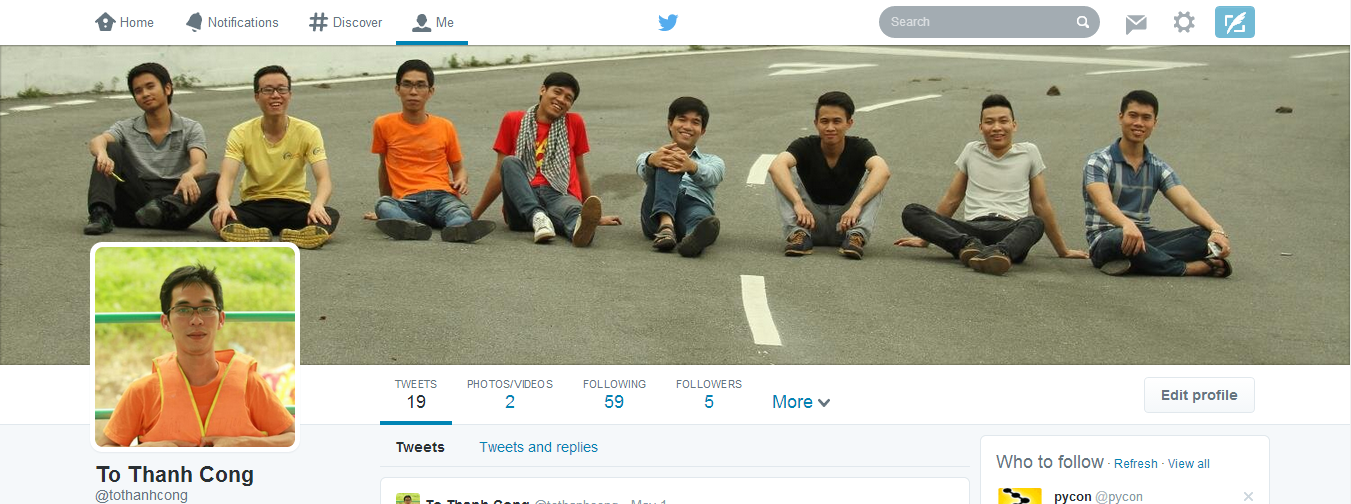
\includegraphics[scale=0.3]{congttwho}
\end{figure}
Tương lai: \Large{\textcolor{red}{\textbf{{OpenStack ... OpenStack ... OpenStack}}}}
\end{frame}
%---Gioi thieu ve nghe quan tri he thon-------------------%
\label{Khi toi noi}
\begin{frame}{2. Khi bạn nói ... mọi người nghĩ ...}
\large{System Administrator / Network Administrator / System Monitor \\
Programmer / PM (Project Manager) / Tester / QA (Quality Assurance)  \\
\textbf{DevOps ....}} \\ 
\framebreak
\pause
\begin{figure}[!ht]
\centering
	\unitlength1cm
			
\includegraphics[scale=0.5]{khibannoi}
\end{figure}
\pause
\textcolor{orange}{\textit{Đừng quan tâm đến việc mọi người nghĩ mà hãy nghĩ về việc mình làm}}
%.......
\end{frame}
%---Cong viec cua quan tri he thong--------------------------%
\label{Python & Cong viec}
\begin{frame}
\frametitle{3. Công việc về hệ thống/mạng}
\pause Triển khai \pause / Vận hành \pause / Hỗ trợ \pause / Sao lưu \& bảo trì \pause / Nâng cấp \& cập nhật ...\\
%..........
\pause
\center{"NO-NAME(VIỆC KHÔNG TÊN)"}
\label{Chu y tai lieu commnent}
\framebreak
\pause
\begin{figure}[!ht]
\centering
	\unitlength1cm
			
\includegraphics[scale=0.5]{automate-all-the-things}
\end{figure}
%..........
\end{frame}
%-----Python danh cho quan tri he thong--------------------%
\label{Slide 1:Python cho Sysad - module os}
\begin{frame}[fragile]
\frametitle{4. Python cho System / Network / (1) }
import os, socket, subprocess \color{gray} $\{$...more...$\}$
\label{import os}
\begin{block}{ipmort os}
\sFontvi
\begin{itemize}
\item Cung cấp các "function", thư viện làm việc với hệ điều hành: Linux / Windows / MAC  \\
\item Bao gồm các việc: thực thi các lệnh / lấy ra thông số trong hệ hiều hành ...
\item Mặc định trong Python
\end{itemize}
\pause
\end{block}
\label{Vi du ve module OS}
\begin{block}{Ví dụ về module OS} 
\Fontvi
%%%%___Bat dau___Chen code python truc tiep%%%%
%\begin{python}
%#!/use/bin/python
%#
%import os
%print os.getcwd() 	#Hien thi duong dan hien tai
%#os.system("tree") 	#Thu hien lenh ls trong Linux
%
%#Tra ve thong tin cua file 
%print "Getting the status of: ", os.stat('D:\Feedback cuoi ky.doc')
%
%##Doi ten cua file	
%print os.rename("D:\Feedback cuoi ky.doc", "D:\phanhoi.doc")
%
%##Hien thi kich thuoc cua file - mac dinh theo bytes
%print os.path.getsize("D:\phanhoi.doc")
%\end{python}
%%%%___KET THUC___Chen code python truc tiep%%%%
%
%%%%___BAT DAU___Chen code python tu file%%%%
\pythonexternal{vidu-os.py}
\end{block}
\end{frame}
%---------Gioi thieu module sys--------------------------%
\label{Slide 2:Python cho Sysad - Module socket}
\begin{frame}[fragile] \label{import socket}
\frametitle{4. Python cho System / Network / (1) }
\begin{block}{ipmort socket}
\sFontvi %thay doi kich thuoc font cua slide
\begin{itemize}
\item Module socket làm việc với các địa chỉ IP, các Port, hostname ....
\item Có thể sử dụng trên cả Windows, Linux ...
\item Mặc định trong Python
\end{itemize}
ref:\\
https://docs.python.org/2/library/socket.html\\
http://pymotw.com/2/socket/addressing.html\\
http://www.pythonforbeginners.com/code-snippets-source-code/python-socket-examples
\end{block}
\end{frame}
%
\begin{frame}[fragile] \label{vi du 1 ve module socket}
\frametitle{4. Python cho System / Network / (1) }
\begin{block}{Ví dụ 1 tổng hợp về module socket} \label{Vi du ve module socket}
\Fontvi
\pythonexternal{vidu-socket.py}
\end{block}
\end{frame}
%
\begin{frame}[fragile] \label{vi du2 ve module socket}
\frametitle{4. Python cho System / Network / (1) }
\begin{block}{Ví dụ 2: Kiểm tra IP của các trang web} \label{Vi du 2 ve module socket}
\Fontvi
\pythonexternal{vidu-socket2.py}
\end{block}
\end{frame}
%------Gioi thieu subprocess-------%
\label{Slide 3:Python cho Sysad - Module subprocess}
\begin{frame}[fragile] \label{import subprocess}
\frametitle{4. Python cho System / Network / (1) }
\begin{block}{import subprocess}
\begin{itemize}
\item Thực thi các lệnh của hệ thống trong Python.
\item Xử lý các subprocess trong hệ thống
\item Làm việc với các input/output/error và trả về kết quả.
\item Thay thế một số modules và functions: os.system, os.spawn*, os.popen*, popen2.* commands
\end{itemize}
ref:\\
https://docs.python.org/2/library/subprocess.html\\
http://www.pythonforbeginners.com/os/subprocess-for-system-administrators\\
http://sharats.me/the-ever-useful-and-neat-subprocess-module.html\\
\end{block}
\end{frame}
%--------------------------------------------------%
\label{Chu y tai lieu commnet 3}
\begin{frame}[fragile] \label{Demo - phan 1}
\frametitle{"Đề Mô" (1)}
%\textcolor{green}{\textit{Đặt mã nguồn chương trình tại đây}}
%%Chen doan 1 cua chuong trinh scanport
\begin{block}{Chương trình Scanport(1)}\label{Chuong trinh scan port phan 1}
\sFontvi
\begin{python}
#!/usr/bin/env python
#Source: http://www.pythonforbeginners.com/
import socket
import subprocess
import sys
from datetime import datetime

# Xoa man hinh trong LINUX
#subprocess.call("clear", shell=True)
# Xoa man hinh trong WINDOWS
subprocess.call("cls", shell=True)

# Nhap dia chi may chu
remoteServer    = raw_input("Nhap may chu can scan: ")
remoteServerIP  = socket.gethostbyname(remoteServer)

# Hien thi ra dong thong bao
print "-" * 60
print "Xin vui long doi, dang Scan may chu ", remoteServerIP
print "-" * 60

# Gan t1 bang thoi gian hien tai
t1 = datetime.now()
\end{python}
\end{block}
\end{frame}
%%%%%%%%%%%%%%%%%%%%%%%%%%%%%%
\begin{frame}[fragile]\label{Demo - phan 2}
%Chen doan 2 cua chuong trinh scanport
\frametitle{"Đề Mô" (2)}
%\textcolor{green}{\textit{Đặt mã nguồn chương trình tại đây}}
\begin{block}{Chương trình Scanport(2)}\label{Chuong trinh scan port phan 2}
\sFontvi
\begin{python}
#Scan tu port 1 toi 1024, dung try ... except de xu ly loi
try:
    for port in range(1,1025):  
        sock = socket.socket(socket.AF_INET, socket.SOCK_STREAM)
        result = sock.connect_ex((remoteServerIP, port))
        if result == 0:
            print "Port {}: \t Open".format(port)
        sock.close()

except KeyboardInterrupt:
    print "Ban da nhan Ctrl+C"
    sys.exit()

except socket.gaierror:
    print "Khong phan giai duoc ten mien, dang thoat ..."
    sys.exit()

except socket.error:
    print "Khong the ket noi den may chu"
    sys.exit()

# Gan thoi gian hien tai bang t2 (sau khi Scan)
t2 = datetime.now()
# Tong thoi gian Scan
total =  t2 - t1
# Hien thi ra man hinh
print "Tong thoi gian Scan la:", total
\end{python}
\end{block}
\end{frame}
%%%%%%%%%%%%%%%%%%%%%%%%%%%%%
%------Cau hinh router -------%
\label{Cau hinh cho route}
\begin{frame}[fragile] 
\frametitle{"Đề-Mô" (3)}
\begin{block}{Cấu hình cho Router} \label{Cau hinh cho Router}
\Fontvi
\begin{verbatim}
R2#sh run
!
hostname R2
!
aaa new-model
!
aaa authentication login VTY enable
!
username cong password 0 123
!
interface FastEthernet0/0
!
interface FastEthernet0/1
 ip address 10.10.10.2 255.255.255.0
!
line vty 0 4
 privilege level 15
 password cisco
 login authentication vty
!
end
\end{verbatim}
\end{block}
\end{frame}
%------Demo telnet va backup router -------%
\label{Demo: Telnet backup router}
\begin{frame}[fragile] 
\frametitle{"Đề-Mô"(4)}
\begin{block}{Mã nguồn: Telnet \& backup cấu hình Router} \label{Ma nguon telnet  backup router1}
\Fontvi
\pythonexternal{vidu-telnet-backup-router.py}
\end{block}
\end{frame}

%------Gioi thieu ve ipython-------%
\label{Slide 4:Python cho Sysad - ipython}
\begin{frame}[fragile] \label{Gioi thieu ipython}
\label{Slide xxx: Gioi thieu ve ipython }
\frametitle{4. Python cho System / Network / (2) }
\begin{block}{Giới thiệu ipython}
Ipython có hai thành phần chính
\begin{itemize}
\item Tương tác với shell (linux) - "Python Shell".
\item Công cụ dành cho xử lý "parallel computing".
\end{itemize}
Làm việc với các hệ điều hành
\begin{itemize}
\item Linux (Centos, Redhat, Ubuntu, Mint ...)
\item Các hệ điều hành tựa Unix (AIX, BSD, Solarix ...)
\item Windows (XP, 7, 8 ...)
\item Mac OS X
\end{itemize}
\end{block}
ref:\\
http://www.pythonforbeginners.com/basics/ipython-a-short-introduction\\
http://ipython.org/documentation.html
\end{frame}
%------Cai dat va su dung ipython--------
\label{Slide xxx: cai dat va su dung ipython}
\begin{frame}[fragile]
\frametitle{4. Python cho System / Network / (2)}
Cài đặt:
\pause
\begin{itemize}
\item Linux: \textit{\textcolor{red}{sudo apt-get install ipython}}
\pause
\item Windows:\textit{\textcolor{red}{pip install ipython}}
\end{itemize}
\pause
Cách sử dụng:
\pause
\begin{itemize}
\item Khởi động: \textcolor{red}{ipython}\pause
\item Sử dụng lệnh của hệ thống : \textcolor{red}{!ping 8.8.8.8}\pause
\item Thực thi chương trình: \textcolor{red}{@run /home/congtt/vidu-ipython.py}
\end{itemize}
\end{frame}
%-------Gioi thieu ve fabric---------------------%
\label{Slide xxx:Python cho Sysad - fabric}
\begin{frame}[fragile]\label{Gioi thieu fabric}
\frametitle{4. Python cho System / Network / (3) }
%\sFontvi
\begin{block}{Giới thiệu về fabric} 
Là thư viện và các công cụ dòng lệnh dùng để tổ chức một cách hợp lý việc triển khai ứng dụng và thực hiện các công việc quản trị hệ thống thông qua SSH. 	
\begin{itemize}
\item Tạo ra các module trong Python chứa một hoặc nhiều funtions và thực thi các module này bằng lệnh \textit{\textcolor{blue}{fab}}
\item Có thể thực hiện các lệnh thông qua SSH.
\end{itemize}
\end{block}
Cài đặt:
\pause
\begin{itemize}
\item Linux: \textit{\textcolor{red}{sudo apt-get install fabric}}
\pause
\item Windows:\textit{\textcolor{red}{pip install fabric}}
\item Kiểm tra: fab -V
\end{itemize}

ref:\\
http://www.pythonforbeginners.com/fabric/how-to-use-fabric-in-python\\
https://github.com/fabric/fabric\\
http://fabfile.org/
\end{frame}
%------Vi du su dung-----------------------------%
\label{Vi du su dung fabric}
\begin{frame}[fragile]
\frametitle{Ví dụ sử dụng fabric}
\sFontvi
\begin{block}{Ví dụ 1:}
Dùng trình soạn thảo tạo mã nguồn dưới và đặt tên là fabfile.py
\pythonexternal{fabfile.py}
\end{block}
\label{Thuc thi file fabric}
\pause
\begin{block}{Thực thi mã nguồn bằng lệnh fab}
\textcolor{red}{fab uptime} (hoặc lệnh) \textcolor{red}{fab host$\_$remote} \\ 
\pause
TIP: \\
thử gõ lệnh \textcolor{red}{fab -l} 
\end{block}
\end{frame}

%-------------------------------------------------%
\label{Tham khao}
\begin{frame}[fragile]
\frametitle{Tài nguyên \& tham khảo.}
\framebreak
\pause
\sFontvi
\textbf{Ebook} \label{Ebook tham khao}
\framebreak
\pause
\begin{itemize}
\item \textit{Python for Unix and Linux System Administration},\textbf{ Noah Gift, Jeremy M. Jones,} O'Reilly Media 2008.
\item \textit{Pro Python System Administration},\textbf{Rytis Sileika}, Apress 2010
\item \textit{Think Python How to Think Like a Computer Scientist},\textbf{Allen Downey}, Green Tea Press
\item \textit{A Byte of Python},\textbf{Swaroop C H}, swaroopch.com
\end{itemize}
%
\framebreak
\pause
\textbf{Cộng đồng \& website}
\framebreak
\pause
\begin{itemize}
	\item http://pythonvietnam.info
	\item http://vithon.org
	\item http://stackoverflow.com/
	\item http://ipython.org/
	\item http://fabfile.org/
	\item http://sites.google.com/site/pythonforlinux/	
	\item http://pythonforbeginners.com/
	\item http://learnpythonthehardway.org/
\end{itemize}
\end{frame}
%----BONUS------------------------------%
\label{Bonus}
\label{Slide: Cach tra tai lieu}
\begin{frame}[fragile]
\frametitle{Cách tra tài liệu}
Cài đặt \& sử dụng pydoc \\ \pause
Cài đặt: \textcolor{red}{\textbf{pip install pydoc}}\\
\begin{block}{Sử dụng}
pydoc os \\
pydoc sys \\
pydoc socket.socket\\ 
.......\\
\pause
\textcolor{red}{\textbf{pydoc -p 8000}}
\end{block} 
\pause
\begin{block}{Windows} 
\begin{verbatim}
C:\python27\Lib\pydoc.py import
\end{verbatim} 
\end{block}
\end{frame}
%---CONG CU KHUYEN CAO-----------------------------%
\label{Slide: Cong cu khuyen cao Notepad++}
\begin{frame}[fragile]
\frametitle{Công cụ khuyến cáo}
\begin{block}{Sử dụng Notepad++ \& VIM}
\begin{itemize}
\item Miễn phí và nhẹ.
\item Có hỗ trợ plugin cho Python.
\item Phím tắt và "gợi ý" từ khóa.
\end{itemize}
\end{block}
\sFontvi
\begin{block}{Cấu hình phím tắt cho Notepad++(WINDOWS)}
Tạo file bat với nội dung sau:
\begin{verbatim}
	@ECHO OFF
	C:\Python27\python "%1"
	echo.
	PAUSE
	@ECHO ON
\end{verbatim}
Lưu thành file với tên là python.bat
\noindent 
\begin{verbatim}
 		C:\Python27\python.bat
\end{verbatim} 
Khai báo phím tắt trong Notepad++ 
\begin{verbatim}
		C:\Python27\python.bat "$(FULL_CURRENT_PATH)"
\end{verbatim}
\end{block}
\end{frame}
%----TRAO DOI VA THAO LUAN-------------------------%
\label{Trao doi & Thao Luan}
\begin{frame}
\frametitle{Trao đổi \& thảo luận}
\Huge{\centerline{Cám ơn sự quan tâm của các bạn !}}
\sFontvi	
	\begin{itemize}
		\item Email: tcvn1985@gmail.com
		\item Twitter: http://twitter.com/tothanhcong
		\item Skype: tu0ng$\_$c0ng
		%\item Phone: 0912349490
	\end{itemize}
\end{frame}
%%%%%%%%%%%%%%%%%%%%%%%%%%%%%%%%%%%%%%%%%%%%%%%%%%%
\end{document}
